\section{Introduction}
The advent of Computer Graphics has \textbf{not replaced artists}. Many non-photorealistic rendering techniques have focused on depicting shape through shading that \textit{mimic hand-drawn illustration} but NPR models still \textbf{lack in expressive power}. \newline
The proposed technique should \textit{correlate} the enhancement functionalities to \textbf{surface feature variations}. To achieve this result, the paper \cite{referencePaper} starts from analyzing two existing techniques that either perturbates the surface normal as in \textbf{Normal enhancement} or alterates reflected radiance based on local surface information as in \textbf{Radiance scaling}. \newline
However, both of those methods have some limitations: \newline 
Normal enhancement operators are \textit{restricted} on specific types of material and illumination models, and they are \textbf{not able to enhance} some important geometry features such as \textbf{concavities} and \textbf{convexities}. In contrary, Radiance scaling overcomes those limitations but (expecially in NPR shading) tends to mask subtle shading variations and hence \textbf{reduce effectiveness} of the overall technique. \newline
The proposed techinque's goal is to \textit{reformulate} NPR shading models with respect to \textbf{geometry surface features} combining the advantages of Normal enhancement and Radiance scaling while also \textbf{relaxing their constraints}. \newline
The enhancement is achieved in two ways. First, by \textit{modifying the surface normal} using a simple high-frequency enhancement operation. Second, by correlating reflected lighting intensity to \textbf{surface curvature} using a new scaling function. \newline
In this way, we can achieve enhacement in diffierent extent, allowing users to produce more desirable enhacement results.

\subsection{Project Overview}
In this project I implemented all the shading models used in \cite{referencePaper} :\newline
\textbf{Blinn-Phong}, \textbf{Cartoon} and \textbf{Gooch} as well as their \textbf{enhanced version}, following the reformulation of the \textit{reflectance radiance equation} described in paragraphs 6.1, 6.2 and 6.3 of \cite{referencePaper}. \newline Contextually, I realized also all the needed \textbf{helping operators}, such as \textit{normal smoothing}, \textit{sharpening} and \textit{curvature} calculation. Lastly, I realized other \textit{subroutines} to better visualize the differences between normal and enhanced normal, as well as curvature and enhanced curvature (that uses enhanced normal). \newline
A list of all the usable subroutine in the project can be seen in \textbf{Figure \ref{fig:all_subroutines}}.

\begin{figure}[h]
	\centering
	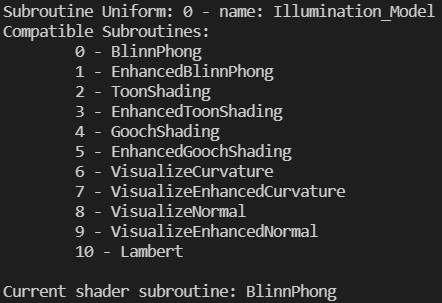
\includegraphics[width=0.5\textwidth]{Images/all_subroutines.jpg}
	\caption{All subroutines available in the project}
	\label{fig:all_subroutines}
\end{figure}